\documentclass[5p, times]{elsarticle}

%%%%%%%%%%%%%%   Preample  %%%%%%%%%%%%%%%%%%

%% The amssymb package provides various useful mathematical symbols
\usepackage{amssymb}
%% The amsthm package provides extended theorem environments
\usepackage{amsthm}
\usepackage{mathtools}

%% for celcius symbol
\usepackage{textcomp}

%% for units
\usepackage{siunitx}

%% The lineno packages adds line numbers. Start line numbering with
%% \begin{linenumbers},  end it with \end{linenumbers}. Or switch it on
%% for the whole article with \linenumbers.
\usepackage{lineno}
\modulolinenumbers[5]

\usepackage{hyperref}

%% package for type Greek letters without entering into math-mode
\usepackage{textgreek}

%% package for large picture in two-colume
\usepackage{dblfloatfix}
\usepackage{fixltx2e}
\usepackage{float}
\usepackage{tabulary}

\usepackage{comment}

%% only jpg pdf eps are allowed, tiff format are not allowed in latex
%% eps in principle can't be compiled by pdflatex, pdf not compiled by latex, but Kile can do some intermedate conversion to allow this happen.
\DeclareGraphicsExtensions{.pdf, .eps, .jpg}
%%opening
\journal{NIMA}

\begin{document}

%%%%%%%%%%%%%% Front Matter %%%%%%%%%%%%%%%%%%
\begin{frontmatter}

\title{Design and verification of a low power large dynamic readout unit for the PSD detector of DAMPE project}

\author[imp,lzu,ucas]{Yong Zhou}

\author[imp]{Yuhong Yu\corref{corresponding_author}}
\cortext[corresponding_author]{Corresponding author}
\ead{yuyuhong@impcas.ac.cn}

\author[imp]{Zhiyu Sun}
\author[imp]{Yongjie Zhang}
\author[imp]{Fang Fang}
\author[imp]{Junling Chen}

\author[lzu]{Bitao Hu}

\address[imp]{Institute of Modern Physics, Chinese Academy of Sciences,  509 Nanchang Road,  Lanzhou,  730000,  P.R.China}
\address[lzu]{School of Nuclear Science and Technology,  Lanzhou University,  222 South Tianshui Road,  Lanzhou,  730000,  P.R.China}
\address[ucas]{Graduate University of the Chinese Academy of Sciences,  19A Yuquan Road,  Beijing,  100049,  P.R.China}

%%
\begin{abstract}

\begin{comment}
A Plastic Scintillator Detector (PSD), consisting of individual 82 organic plastic scintillator strips with 1 cm thick,
located at the top of DAMPE (DArk Matter Particle Explore), has been developed. It mainly serves as anti-coincidence
detector, also as a charge detector to measure cosmic ray nuclei up to charge $Z=20$. A large dynamic range from \SI{0.1}{MIPs} to \SI{1400}{MIPs} has been deduced after consideration various contributions. 
Integrating of a PMT with double dynodes readout and an ASIC chip VA160, a large dynamic readout system has been presented. 
A cosmic ray muons and an accelerator beam test have been used to verify this design, respectively. 
The results show that the readout system could satisfy the required dynamic range. 
\end{comment}

A large dynamic range readout unit is developed for the Plastic Scintillator Detector(PSD) of DArk Matter Paricle Explorer(DAMPE).
By extracting the signal form dynode5 and dynode8 of the photomultiplier tube, the unit can cover the wide signal amplitude range of PSD(from electron to Z=20).
The design has been verified using cosmic ray muon and relativistic Ar beam at CERN.
A dynamic range from \SI{0.1}{MIPs} to \SI{1400}{MIPs} has been achieved.

\end{abstract}

%%
\begin{keyword}
plastic scintillator
\sep VA160
\sep large dynamic range
\sep double dynodes readout

%% PACS codes here,  in the form: \PACS code \sep codes

\end{keyword}

\end{frontmatter}

\linenumbers
%%%%%%%%%%%%%%%%  Introduction  %%%%%%%%%%%%%%%%%%%%%%%
\section{Introduction}
\label{sec:introduction}

DArk Matter Paricle Explorer(DAMPE) is a satellite-borne particle detector aiming for in-direct dark matter search, high-energy gamma astronomy and primary cosmic ray study~\cite{Chang_Jin_dampe}.
It is designed to cover a wide energy range, from \SI{5}{GeV} to \SI{10}{TeV} for electrons and photons and from \SI{10}{GeV} to \SI{1}{PeV} for heavy ions, with unprecedented resolution(\SI{1.5}{\percent} at \SI{100}{\giga\electronvolt}).
% By extending the measurement to the \si{TeV} region, DAMPE will complement current experimental results~\cite{guzik_advanced_1999,picozza2010instrument,aguilar2013first} and shed more light on the new phenomena in this region. 
The Plastic Scintillator Detector(PSD), which sits at the top of the satellite, is a key sub-detector of DAMPE.
It consists of two layers of plastic scintillator bars which are orthogonal to each other, and covers an effective detection area of $\SI{820}{mm}\times\SI{820}{mm}$.
The bars are made of EJ-200~\cite{scintillator} with the dimension of $\SI{884}{mm} \times \SI{28}{\milli\meter} \times \SI{10}{mm}$, and coupled to a Hamamatsu R4443 PMT~\cite{r4443} at both ends.
% using \SI{3}{mm}-thick silicon rubber(EJ-560~\cite{scintillator}).

\begin{comment}
To fulfil the requirements and optimize performance, the readout unit of PSD needs a careful design, which is guided by the following rules:
\begin{itemize}
 \item Large dynamic range.To cover the signal amplitude from minimum ionizing electrons to relativistic calcium ions.
 \item Large signla-to-noise ratio(SNR).For efficient charged particle detection.
 \item Low power consumption. The whole PSD is limitted to 19W, 12W for the front end electronics and 7W for the detection units(high voltage distribution and PMT base circuit).
\end{itemize}
\end{comment}
By measuring the deposited energy, PSD serves as an anti-coincidence detector for e/$\gamma$ discrimination as well as a charge detector for heavy ions up to Z=20.
These functions impose harsh demands for the readout system of PSD, which, together with the PMT, needs to cover a wide range of signal amplitudes from singly charged minimum ionizing particles to relativistic calcium ions, while in the same time keeping sufficient resolution and large signal-to-noise ratio(SNR) for effective particle identification.   
As a space experiment, the power consumption of PSD is restricted to be $\leq$19W as a whole, 12W for the front end electronics(FEE) and 7W for the high voltage distribution and PMT base circuit.
This adds an extra constraint in the design of the readout unit.

In this paper, a low power and large dynamic range readout unit for PSD is reported.
Verification tests for the design have been carried out using cosmic ray and relativistic heavy ion beam, and the results are satisfactory.
The detailed description of the design is presented in Sec.\ref{sec:requirement} and Sec.\ref{sec:design}, and the test results are discussed in Sec.\ref{sec:result}.

%%%%%%%%%%%%%%%% Main Text Body %%%%%%%%%%%%%%%%%%%%%%%
\section{Dynamic range requirement}
\label{sec:requirement}

\begin{figure*}
\centering
 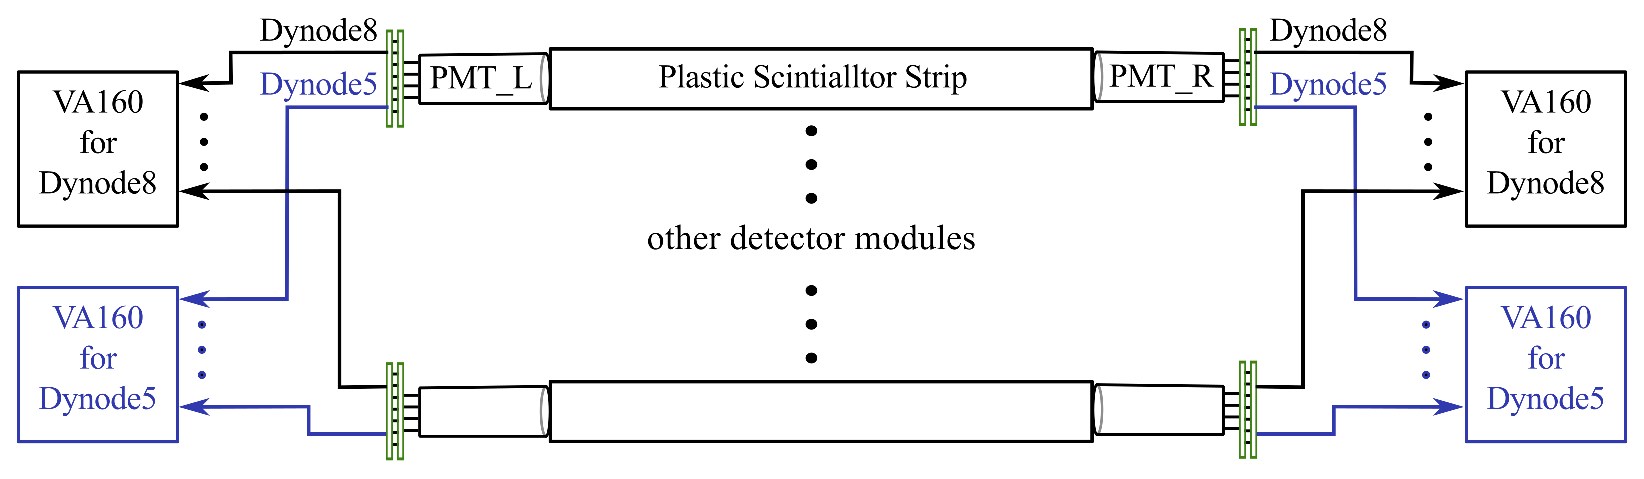
\includegraphics[width=140mm]{readout_scheme}
\caption{Readout scheme of PSD.}
\label{fig:readout_scheme}
\end{figure*} 

\begin{figure*}
\centering
 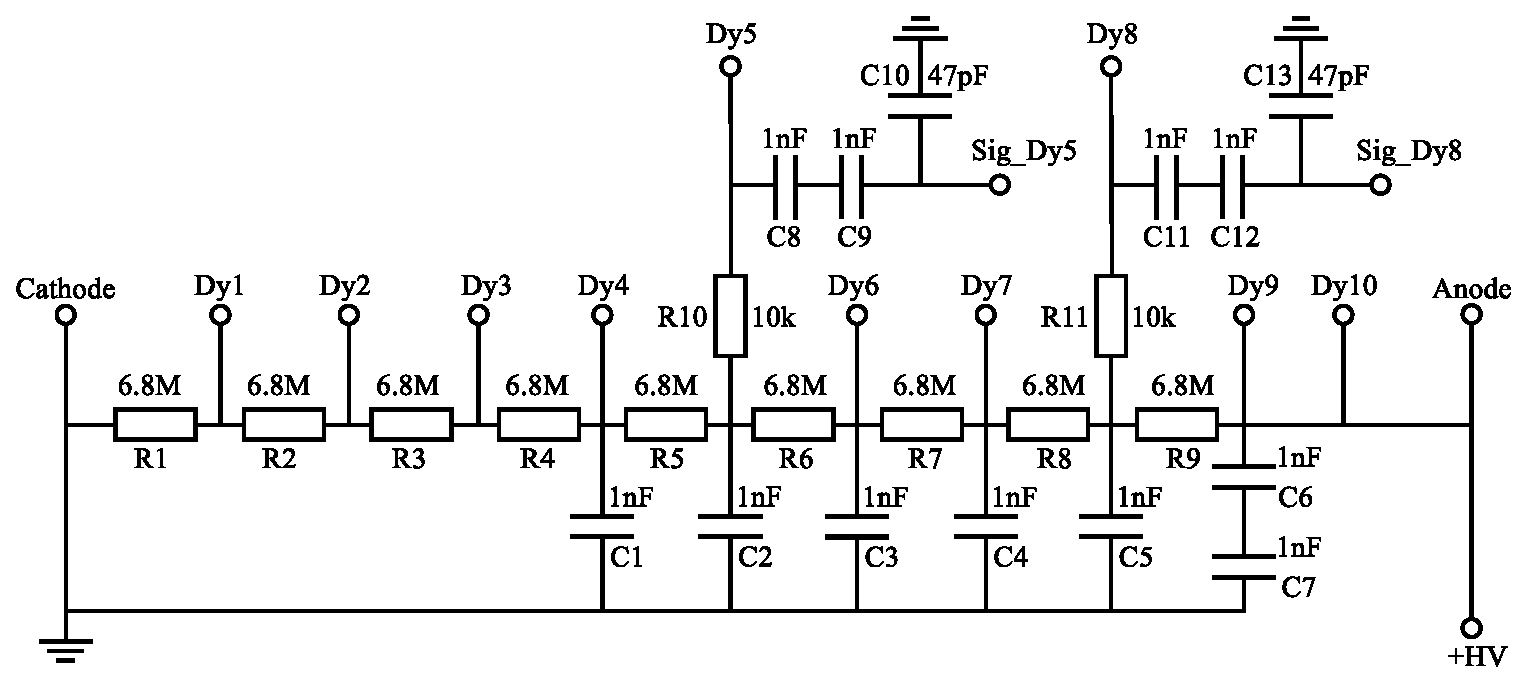
\includegraphics[width=130mm]{divider}
\caption{Circuit diagram of the voltage divider.}
\label{fig:divider}
\end{figure*} 

\subsection{Light yield in response to relativistic heavy ions}
\label{sec:light_yield}
% According to the Bethe-Bloch equation~\cite{olive_review_2014}, the energy deposited in PSD bars is approximately proportional to $Z^2$ for particles heavier than electron.
The light yield of organic scintillator is a nonlinear function of the desposited energy $\Delta E$ due to the quenching effect.
It can be described precisely by the Birks law~\cite{birks_theory_2013} in the low energy range, while for heavy ions in the relativistic region, the scintillation mechanism gets much more complicated and the Birks law fails to apply.
Several modified models~\cite{chou_nature_1952,tarle_cosmic_1979,menchaca-rocha_response_1999,matsufuji_response_1999} have been proposed to extend the Birks law to the high energy region, nevertheless large discrepancy exists between them when extrapolating to the high-Z nuclides.

Due to the theoretical difficulties metioned above, our estimation of the light yield is based on the direct beam test result of AMS-02 TOF prototype~\cite{bindi2005performance}, which also uses EJ-200 as the detection material and has the same thickness.
According to ~\cite{bindi2005performance}, the light output of calcium is about 270 times larger than that of proton.
As all singly charged minimum ionization particles have approximately the same response in the plastic scintillator, this result indicates a maximum of 270 times difference in the light yield for all the particle species covered by PSD.

\subsection{Miscellaneous contributions to the dynamic range}
\label{sec:misc_contributions}
Actual dynamic range needed by PSD readout system is expanded by several other contributions. 
To make things clear, we define the mean light yield produced by a singly charged minimum ionizing particle penetrating vertically through the middle of the bar as one MIP, and use it as the unit for the dynamic range calculation.

The first contribution comes from DAMPE's broad field of view, which implies a maximum incidence angle of \SI{60}{\degree} for particles through PSD.
This doubles the travel length and the energy deposit in the bar, and expands the maximum light yield to \SI{540}{MIPs}.  
Secondly, the statistical nature of the ionizing process should be taken into account.
Assuming a full coverage of the energy fluctuation is 5$\sigma$ and $\sigma$=\SI{10}{\percent}, the dynamic range of light output expands to \SI{675}{MIPs} in the upper limit and \SI{0.75}{MIPs} in the lower limit. 
Finally, the long length of the scintillator bar makes the light attenuation non-negligible.
The bars are surface-polished and wrapped by the Tyvek paper~\cite{tyvek} to improve reflection efficiency, and preliminary tests show that the light reduction ratio between the middle position and the two ends can be well controlled above 0.5.
Thus, the light collected by the end PMTs will vary between \SI{0.375}{MIPs} and \SI{1350}{MIPs}.

To leave some redundancy for the adjustment, the final dynamic range demand for the readout unit of PSD is determined to be \SI{0.1}{MIPs}$\sim$\SI{1400}{MIPs}.

\section{Design of the readout unit}
\label{sec:design}
% Power consumption and robustness are the major concern in the design of a readout unit for space usage.
\begin{figure*}[b]
 \centering
 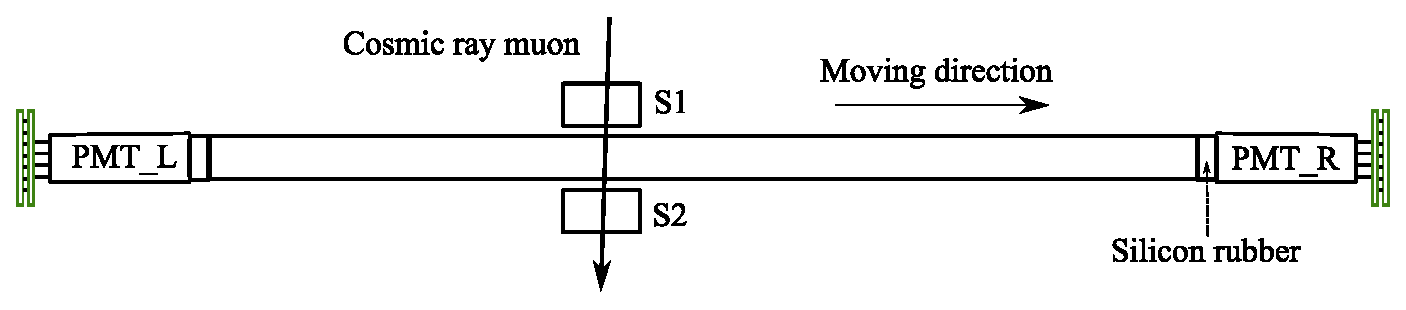
\includegraphics[width=130mm]{cosmic_test}
\caption{The experimental setup for the cosmic ray test.}
\label{fig:cosmic_test}
\end{figure*} 

\subsection{Readout scheme}
\label{sec:scheme}
The ASIC chip VA160, which is developed by IDEAS~\cite{va160} and optimized for the DAMPE project, is adopted as the major signal processing circuit for the charge measurement of PSD.
% due to its low power consumption, high channel integration and successful applications in space usage~\cite{alcaraz_alpha_}.
VA160 is a low power and radiation harden ASIC with a dynamic range from \SI{-5}{\pico\coulomb} to \SI{13}{\pico\coulomb}. 
It integrates 32 input channels into a single chip, and each channel consists of a full chain of charge sensitive pre-amplifier, shaping amplifier and sample-and-hold circuit.
% The high integration level allows compact design of .
% Thus, current pulses from R4443 can be connected to VA160 directly, and the output will be digitized by a 14 bits ADC.

A single VA160 channel is not sufficient to cover the full dynamic range required by PSD.
We adopt the readout scheme of extracting signals from two dynodes of R4443 and then connecting them to separate VA160 channels.
Two measurement ranges can be achieved in this way, with the high gain dynode channel for small light output measurement and the low gain dynode channel for large light output measurement.
While alternative methods exist~\cite{katayose2008development,kampert1994high,genolini_low_2003}, this readout scheme is preferred because the largest SNR can be achieved without adding extra active electronic components, which in turn implies low power consumption and robustness.
To reduce the crosstalk effect, signals from the two dynodes are connected to different VA160 chips as shown in Fig.\ref{fig:readout_scheme}.

FEE board based on VA160 has been developed and fully tested~\cite{fee}. Outputs from VA160 are digitized by a 14 bits ADC.
A linear range up to \SI{12}{\pico\coulomb} is guaranteed for each FEE channel, and the mean RMS electronic noise is about \SI{4}{\femto\coulomb}. 
The electronic noise level determines the lower limit of the dynamic range.
Assuming the maximum noise level is \SI{50}{\percent} larger than the typical value and 5$\sigma$ is needed to separate signal from noise, this implies the response of \SI{0.1}{MIPs} shall be larger than \SI{30}{\femto\coulomb}, i.e. 1MIPs$\geq$\SI{300}{\femto\coulomb}.
Hence the maximum dynamic range covered by the high gain dynode channel is \SI{0.1}{MIPs}$\sim$\SI{40}{MIPs}, and the remaining range shall be covered by the low gain dynode channel.
This constrains the gain ratio between the two dynodes to be $\geq$35.

\subsection{Selection of the dynode stages}
\label{sec:dynodes_selection}
To determine the appropriate dynode stages for readout, an estimation of the mean number of photon electrons(PE) generated by one MIP in the middle of the bar is carried out.

The mean energy deposit of the MIP particle in a \SI{10}{\milli\meter} plastic scintillator is about \SI{2.0}{\mega\electronvolt}~\cite{olive_review_2014}, and the scintillation efficiency of EJ-200 is \SI[per-mode=symbol]{e4}{photons\per\mega\electronvolt}~\cite{scintillator}.
Light output is distributed to both ends of the bar equally.
However, only \SI{22.5}{\percent} of the generated photons are within the total reflection angle and will undergo the transmission process to the end of the bar, due to the refraction on the boundary surface.
The final number of photon electrons is calculated as follows:
\begin{align}
 N_{PEs} &= \frac{1}{2} \times \SI[per-mode=symbol]{2}{\mega\electronvolt} \times \SI{e4}{\per\mega\electronvolt} \times 0.225
           \times \varepsilon_{1} \times \varepsilon_{2} \times \varepsilon_{3} \times \varepsilon_{4} \nonumber \\
         &\approx \SI{45}{e^-\per{MIP}}
\label{eq:pes}
\end{align} 
where $\varepsilon_1$($\geq$0.5) is the light attenuation ratio caused by the transmission loss from the middle position to the end of the bar,
$\varepsilon_2$($\approx$0.3) is the the geometry factor induced by the effective coupling area between R4443 input window and the bar's end surface,
$\varepsilon_3$($\approx$0.9) is the transmission coefficient of the silicon rubber which is the coupling material between R4443 and the bar,
and $\varepsilon_4$($\approx$0.15) is the quantum efficiency of R4443 cathode.
%The value of $\varepsilon_1$ is based on the measurement results~\cite{zhangyj_scintillator}, $\varepsilon_2$ is the calculation result of the effective coupling area divided by the end surface area, $\varepsilon_3$ and $\varepsilon_4$ are from the datasheets.

R4443 is a 10-stage PMT with a gain of $1\times10^6$ at the typical supply voltage using standard voltage divider(i.e. equal voltage drop between dynodes).
A simple calculation shows that the multiplication factor between adjacent dynodes is about 4.
Combining this result with the estimated PE numbers from Eq.~\ref{eq:pes}, dynode 5 and 8 are selected as the readout composition, which corresponds to a typical MIP response of \SI{450}{\femto\coulomb} and a gain ratio of 65.
The figures are both higher than the desired value, thus the supply voltage need to be lowered to get the optimal result.
The composition of dynode 5 and 7 with higher voltage supply is an alternative choice, it is dismissed because this increases power consumption, reduces the adjustment flexibility and may even exceed the allowed PMT operation voltage in the worst case.

\subsection{Voltage divider circuit}
\label{sec:divider_design}
A cathode grouding voltage divider circuit, which can extract current pulses from both dynode 5 and 8, is designed as shown in Fig.\ref{fig:divider}.
The uniform voltage distribution ratio is adopted instead of the tapered one, because R4443 is a small size tube and the space charge effect at dynode 8 is not an issue at the PSD light intensity level.
To retain the voltage ratio between the latter dynodes and in turn improve linearity, the parallel decoupling capacitors C1$\sim$C7 are added to compensate the charge required in the formation of large signals.

As positive high voltage is supplied, coupling capacitors are needed in the dynode readout branch circuits.
Two serial-chained capacitors(C8/C9 and C11/C12) are used in each branch to provide robustness, in case that one of them breaks down and the other can still protect the following circuits.  
The ramping resistors R10/R11 and bypass capacitors C10/C13 are added to better form the output pulse shape.

Finally, signals from dynode 5 and 8 are connected to the FEE board using coaxial cables to reduce the crosstalk effect between them.

\section{Tests result}
\label{sec:result}
Based on the design described above, a prototype of the PSD detector module has been developed and a series of tests have been carried out to check the performance of the readout unit.

\subsection{Test with LED}
\label{sec:led}
Before coupling to the plastic scintillator bar, the linearity between the dynode 5 and 8 of the readout unit is verified using a blue LED source.
By varying the light intensity of the LED in a large range, the correlation between dynode 5 and 8 can be recorded as shown in Fig.~\ref{fig:linearity}.
A perfect linearity is achieved until the saturation of dynode 8.
Several voltage values from \SIrange{700}{1000}{\volt} have been applied to the voltage divider, and the non-linearity is less than \SI{0.1}{\percent} in all the cases. 

%The gain ratio between dynode 8 and 5 has been extracted at each supplying voltage and the dependency is fitted quite well with the power law function.
%This result will be compared with the cosmic ray measurement result described in the next section.

\begin{figure}
\centering
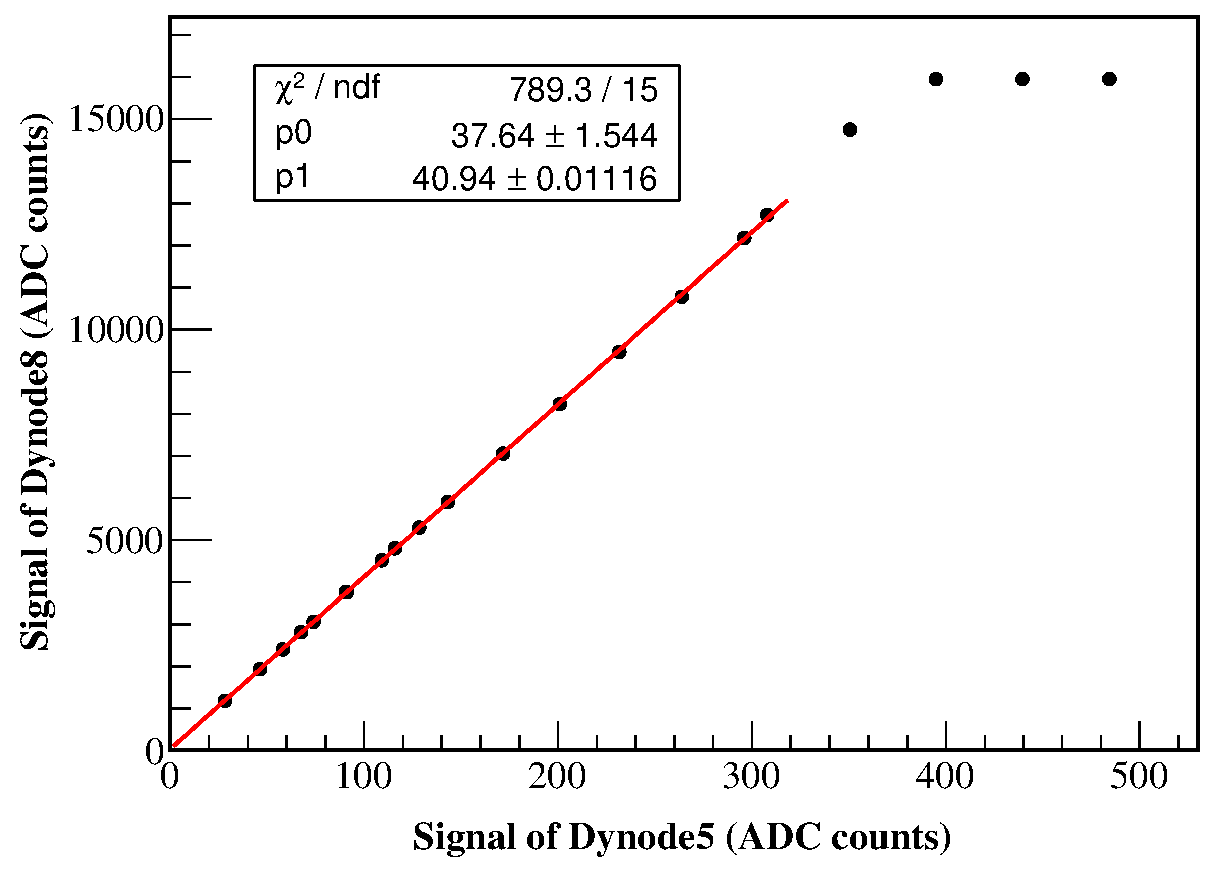
\includegraphics[width=90mm]{linearity}
\caption{Linearity between dynode 5 and 8}
\label{fig:linearity}
\end{figure}


\subsection{Test with cosmic ray}
\label{sec:cosmicray}
Cosmic muons at the sea level are perfect minimum ionizing particle source, hence can be used to study the MIPs response of PSD detector module in the laboratory.
The layout of the test setup is shown in Fig.~\ref{fig:cosmic_test}.
Two coincidence detectors(small plastic scintillator blocks, $\SI{20}{mm} \times \SI{10}{\milli\meter} \times \SI{10}{mm}$), one above and the other below the PSD bar, are used to tag the vertically incident cosmic ray.
Both detectors are fixed on a movable stage, and can move along the bar direction to investigate the response difference at various positions. 

The supplying voltages of R4443 are first adjusted to get the designed MIPs response in the middle of the bar as described in Sec.~\ref{sec:dynodes_selection}.
The result from one end of the PSD detector module is shown in Fig.\ref{fig:mip}, the spectrum follows the Landau distribution and the most probable value is 395.8 ADC counts corresponding to \SI{366}{\femto\coulomb} when converted to charge.
By fitting the lower half of the MIPs peak using Gaussian distribution, the relative resolution is found to be about \SI{16.6}{\percent}.
The pedestal spectrum of this readout channel is also shown in the figure, and the RMS noise level is 5.8 ADC counts(\SI{5.4}{\femto\coulomb}), which implies the lower limit of the dynamic range for this readout channel is about \SI{0.09}{MIPs}.

The MIPs measurements are then carried out every \SI{10}{\centi\meter} along the bar.
The relative light output at each position is shown in Fig.~\ref{fig:attenuation}, and the data can be described precisely by the following model~\cite{taiuti_measurement_1996}:
\begin{equation}
A(x)=C_0(e^{-x/\lambda} + \alpha e^{(2L-x)/\lambda})
\end{equation} 
where L is the total length of the bar, $\alpha$ is an empirical factor related to the fraction of photons reflected back from the far end of the bar and adding to the light intensity at the near end.
Based on the fitting result, the light attenuation ratio at various positions can be calculated(see Tab.~\ref{tab:summary}) and they are all within the estimation limit described in Sec.~\ref{sec:requirement}.
The SNR of the readout unit can also be derived combining all the measurement results above, and they are larger than 10 for both ends of the PSD detector module.

The gain ratio between dynode 8 and 5 can be extracted from the cosmic ray test by combining data from all tested positions.
The result from one end of the bar is shown in Fig.~\ref{fig:dy58}, and the gain ratio is determined to be 44.6 by using a linear fit, which is consistent with the LED test result.
Hence, the upper limit of this readout unit is estimated to be \SI{1462}{MIPs} and fulfills the requirements of \SI{1400}{MIPs}.


\begin{table*}
	\centering
	\caption{Summary of the measured parameters of both ends of the PSD detector module}
	\label{tab:summary} 
\begin{tabulary}{140mm}{|c|c|c|c|c|c|c|c|}
	\hline  & MIPs(mpv) & MIPs($\sigma$) & Noise Level($\sigma$) & Light Attenuation(mid/min) & Dy8/Dy5 & $^{40}Ar$(mean) & $^{40}Ar$(sigma) \\ 
	\hline Left End &  &  &  &  &  &  &  \\ 
	\hline Right End &  &  &  &  &  &  &  \\ 
	\hline 
\end{tabulary}
\end{table*}

\begin{figure}
	\centering
	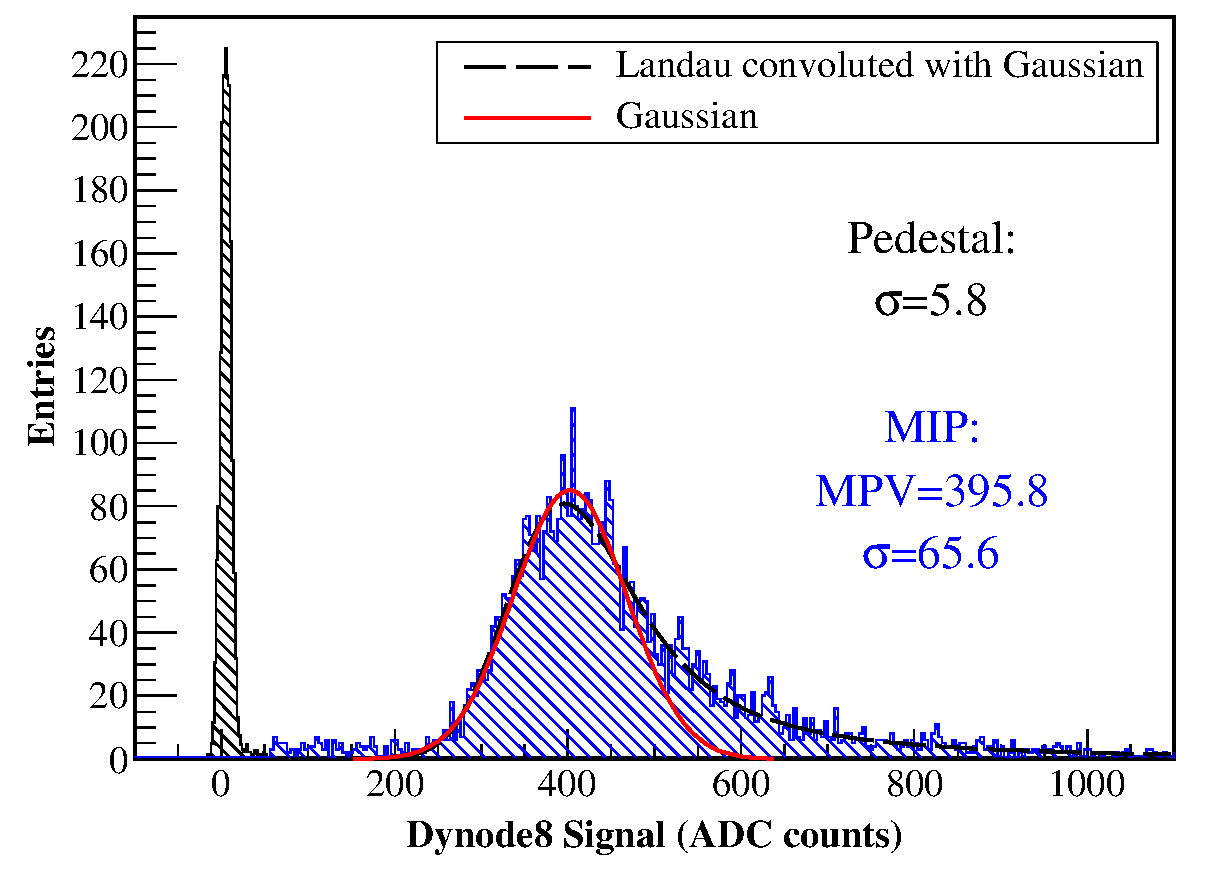
\includegraphics[width=90mm]{mip}
	\caption{The pulse height distribution of cosmic muons from a low gain channel Dy8.}
	\label{fig:mip}
\end{figure} 

\begin{figure}
	\centering
	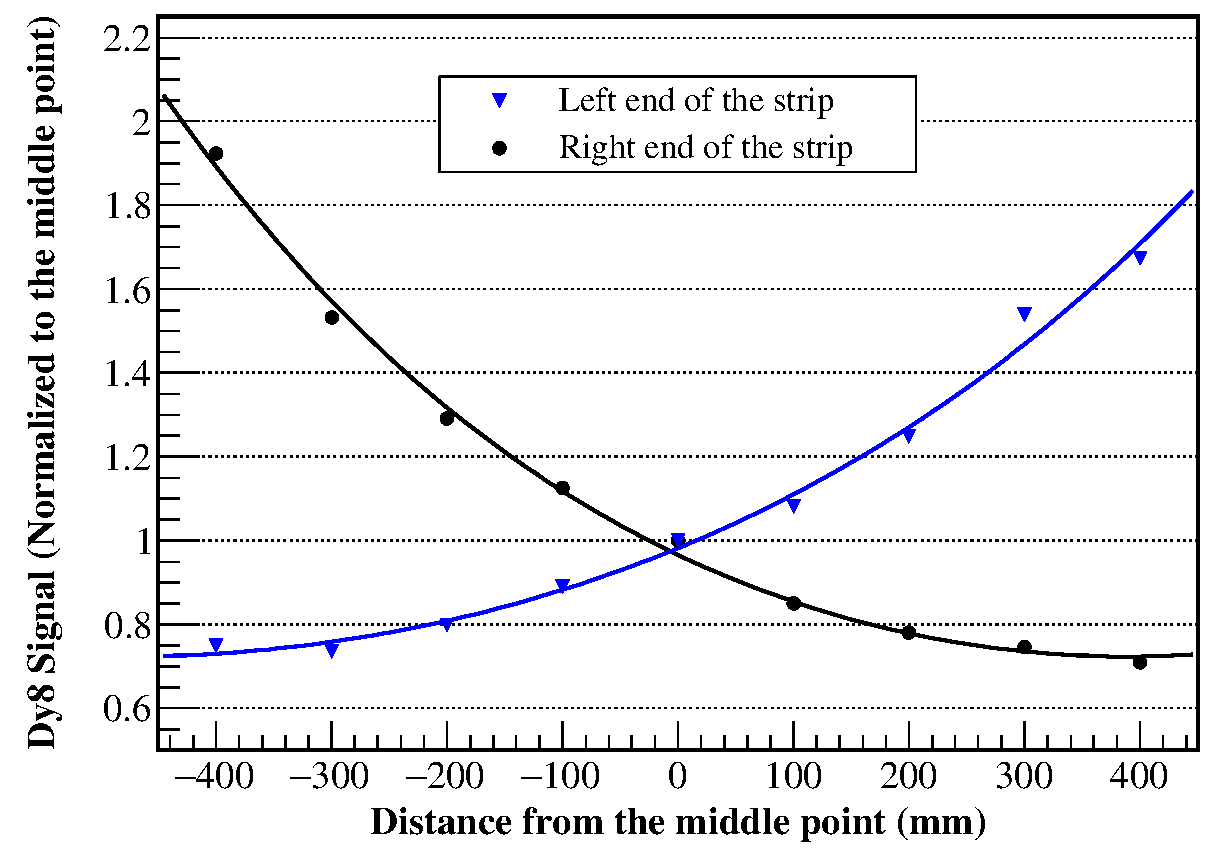
\includegraphics[width=90mm]{attenuation}
	\caption{The charge pulse amplitude at different hit positions along the tested scintillator strip.}
	\label{fig:attenuation}
\end{figure} 

\begin{figure}
	\centering
	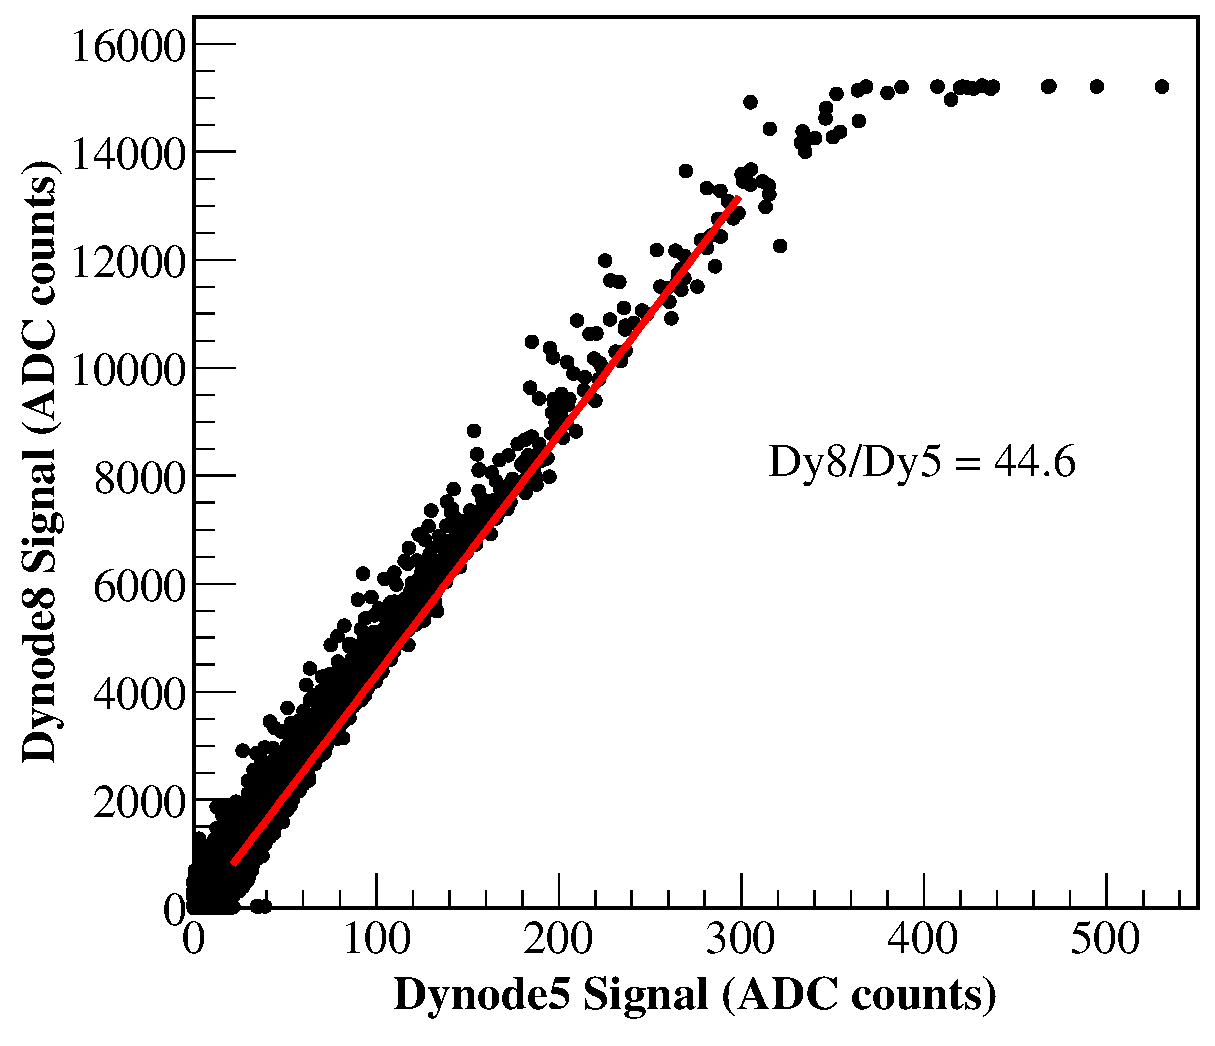
\includegraphics[width=90mm]{dy58}
	\caption{The correlation between the signals in a low gain channel Dy8 and a high gain Dy5.}
	\label{fig:dy58}
\end{figure} 

\subsection{Test with relativistic heavy ion beam}
\label{sec:beam}
To verify the upper limit of the readout dynamic range, a heavy ion beam test is carried out at the H8 beam line of CERN SPS, April 2015.
A primary $^{40}{Ar}$(Z=18) beam of \SI{40}{AGeV\per c} is extracted from SPS and impinging on the middle of PSD's plastic scintillator bar.
During the beam test, the same supply voltage as determined from the cosmic ray test described in Sec.\ref{sec:cosmicray} is applied for direct comparison.
  
As expected, the signal recorded by dynode 8 of the readout unit has already saturated and only dynode 5 can be used for energy measurement.
The ADC spectrum recorded by dynode 5 of one side of the bar is shown in Fig.\ref{fig:Ar}. 
The long tail before the primary $^{40}Ar$ peak corresponds to lighter nuclei which are the products of $^{40}Ar$ interacting in other detectors in front of PSD detector module.
Using the Gaussian distribution, the mean value of $^{40}Ar$ peak is determined to be 1921 ADC counts which corresponds to \SI{217}{MIPs}, and the resolution is about \SI{4.2}{\percent}.
This result is quite consistent with the AMS-02 TOF's result of \SI{210}{MIPs}~\cite{bindi2005performance}, hence validates our previous estimation of light yield in Sec.\ref{sec:requirement}.

An extrapolation based on the simple $Z^2$ dependency(i.e. without considering the quenching effect) gives that the response of Ca in the middle of the PSD bar shall be about \SI{268}{MIPs}, which corresponds to 2372 ADC counts in dynode 5.
Assuming the resolution of Ca to be \SI{5}{\percent} and taking into account other effects described in Sec.\ref{sec:requirement}, the largest signal in dynode 5 will be about \SI{1206}{MIPs}(), which is well within our design limit of the dynamic range.
The other side of the bar has similar results.
%Thus, our design of the readout unit of PSD can fulfill the requirement 

\begin{figure}
 \centering
 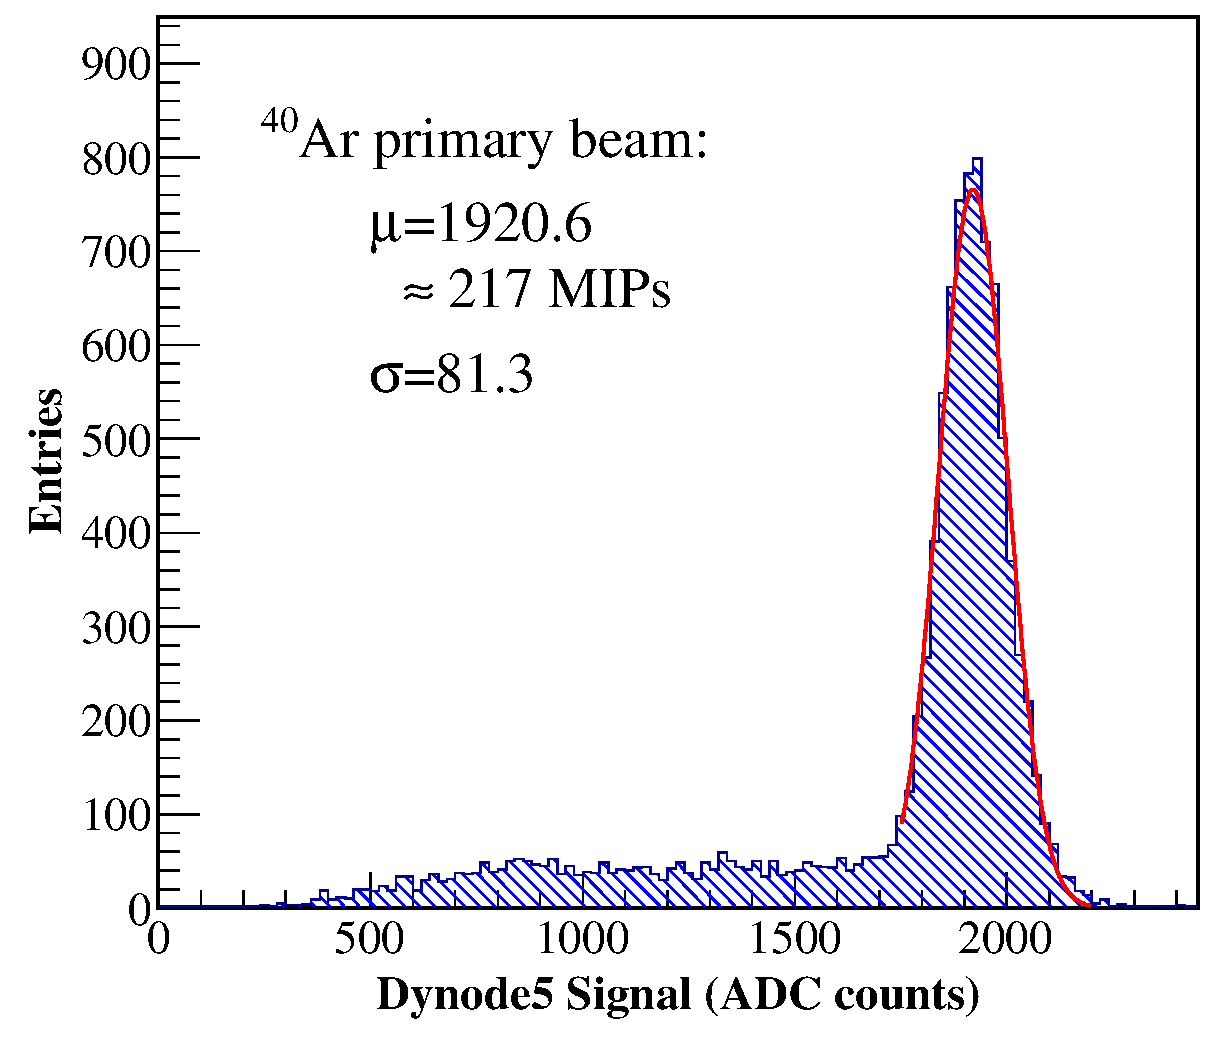
\includegraphics[width=90mm]{Ar}
\caption{The energy deposition distribution from a relativistic $^{40}Ar$ beam.}
\label{fig:Ar}
\end{figure} 

\section{Conclusion}
\label{sec:conclustion}

A broad energy dynamic range of 0.1 MIPs$\sim$1400 MIPs required for each PSD has been deduced from a number of contributions, including energy deposition of nuclei up to charge $Z=20$, light attenuation, particle incidence angle and fluctuation of energy loss. 
A readout system that used a PMT with double dynodes output coupled to FEE with a chip VA160 optimized for positive polarity signals has been developed and used to measure the energy deposition in a scintillator strip. 
Cosmic ray muons were used to investigate the influence of scintillation light attenuation, MIPs peak and the equivalent noise of the whole detector system. 
The input noise of the whole PSD system is approximately \SI{3}{\femto\coulomb}, and the most probable value of the signal-to-noise is greater than 10 for the lower signals with 0.1 MIPs energy deposition. 
It’s also found that the required upper dynamic range 1400 MIPs could be covered by our design easily. 
A relativistic argon beam test has been also used to verify the design. 
Once again the result shows that the readout system could satisfy the large dynamic range requirements.

\subsection{summary}
power consumption
dynamic range

\subsection{production suggestions}
test of pmt
selection of scintillator bar

%%%%%%%%%%%%%%%% Acknowledgement %%%%%%%%%%%%%%%%%%%%%%%
\section*{Acknowledgement}
\label{sec:acknowledgement}

This work was supported by the Strategic Priority Research Program on Space Science of the Chinese Academy of Science,
Grant No. XDA04040202- 3. The authors wish to thank all the people from DAMPE collaboration who helped make this work
possible.

%%%%%%%%%%%%%%%%   Bibliography  %%%%%%%%%%%%%%%%%%%%%%%
%% bibliography style
\section*{References}
\label{sec:reference}
\bibliographystyle{elsarticle-num}

%% From BibTex file
\bibliography{mybib}

\end{document}

\endinput




